\chapter{Validazione del Framework}
\lhead{Validazione del Framework}
In questo capitolo verrà brevemente discusso il processo di validazione del Framework. 

\section{Introduzione}
\rhead{Introduzione}
Durante la fase di sviluppo il Framework è stato testato con applicazioni create ad hoc che permettessero di poter agilmente riprodurre specifiche casistiche, senza dover ogni volta cercare bug di applicazioni che riproducessero la situazione desiderata. Al termine dello sviluppo, per garantire che lo strumento funzionasse anche con applicazioni reali, è stata effettuata una breve validazione. I bug utilizzati per il processo sono stati selezionati tra quelli individuati dal collega D. Triolo nella sua relazione di laurea triennale. Focus della validazione sono le funzioni di: automazione dei test, cattura del  risultato e verifica della riproduzione del bug. Per questo motivo non è stata posta attenzione alla funzione di offuscamento dei dati, già validata da altri colleghi.
\newpage
\section{Applicazioni}
\rhead{Applicazioni}
\subsection{ActivityDiary}
 \begin{figure}[H]
	
\includegraphics[width=3.35cm]{activity.diary}
	\centering
\end{figure}

\noindent\textbf{Introduzione}\newline
Activity Diary è un’applicazione che consente di registrare le proprie attività personalizzandole con note e foto.\\ (\textcolor{gray}{repository: }https://github.com/ramack/ActivityDiary)
\\\\
\noindent\textbf{Bug}\newline
Nella relase 0.4, l’inserimento di un’attività con nome già esistente nell’elenco, provoca un crash dell’applicazione.
\\\\
\noindent\textbf{Caso di test}\newline
Il caso di test prevede l'inserimento di due attività, i cui nomi sono stati resi parametri (\emph{activityName1}, \emph{activityName2}). 
\\\\
\noindent\textbf{Riproduzione del bug}\newline
\noindent\ul{tipologa del bug atteso:} crash\\
Se l’app termina con un crash allora il bug è riprodotto.
\\\\
\noindent\textbf{Validazione}
 \begin{figure}[H]
	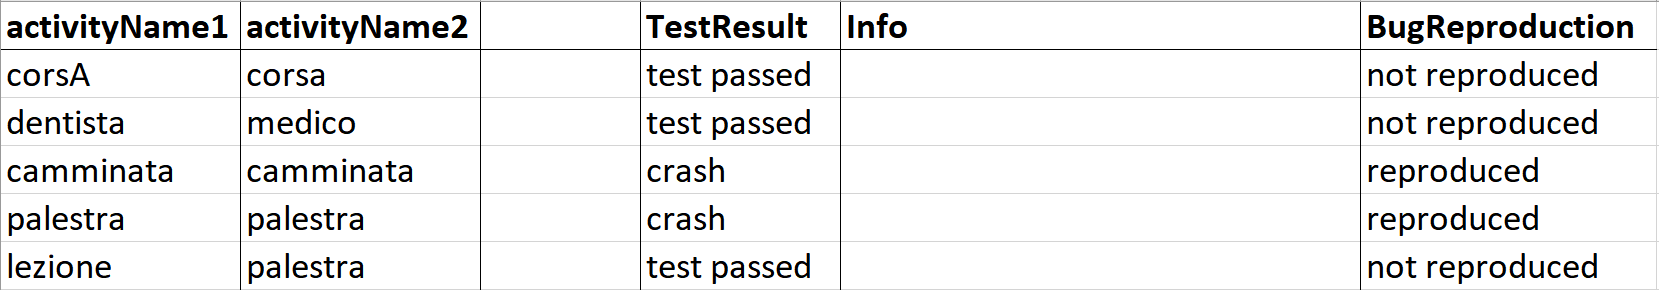
\includegraphics[scale=0.35]{activity.diary.out}
	\centering
				\caption{\emph{output.csv}}
    \label{fig:activity.diary}
\end{figure}
\noindent Come visibile in Figura \ref{fig:activity.diary}, il Framework considera correttamente il bug riprodotto (BugReproduction='reproduced') quando l'esecuzione del caso di test parametrico fa terminare l'applicazione con un crash (TestResult="crash"). Nell'esempio considerato infatti,  quando il caso di test prevede l'inserimento di 2 attività con lo stesso nome (caso [\emph{activityName1="camminata"}, \emph{activityName2="camminata"}], caso [\emph{activityName1="palestra"}, \emph{activityName2="palestra"}]), l'applicazione termina con un crash e il bug viene riprodotto. Quindi l'attività di validazione per questo specifico caso è andata a buon fine.

\subsection{PrivacyFriendlyShoppingList}
 \begin{figure}[H]
	
\includegraphics[width=3cm]{shopping.list}
	\centering
\end{figure}

\noindent\textbf{Introduzione}\newline
PrivacyFriendlyShoppingList è un’applicazione che consente di creare liste della spesa e gestirle aggiungendo, modificando e eliminando oggetti e liste stesse.\\ (\textcolor{gray}{repository: }https://github.com/SecUSo/privacy-friendly-shopping-list)
\bigskip\newline
\noindent\textbf{Bug}\newline
Nella relase 1.0.5, il click del tasto “-“ al momento della creazione dell’item, senza aver inserito un valore nel campo del numero di occorrenze del prodotto, provoca un crash dell’applicazione.
\bigskip\newline
\noindent\textbf{Caso di test}\newline
Il caso di test prevede l'inserimento di una nuova lista con specifica del nome (parametro \emph{listName}) in cui viene aggiunto un nuovo item con specifica del nome (parametro \emph{productName}). Prima di terminare l'aggiunta dell'item, senza aver inserito nessun valore nel campo del numero di occorrenze, viene effettuato un click sul tasto '-'.
\bigskip\newline
\noindent\textbf{Riproduzione del bug}\newline
\noindent\ul{tipologa del bug atteso:} exception (expectedException: 'java.lang.NumberFormatException')\\
\noindent Se l'applicazione solleva l'eccezione 'java.lang.NumberFormatException', allora il bug è stato riprodotto.
\bigskip\newline
\noindent\textbf{Validazione}
 \begin{figure}[H]
	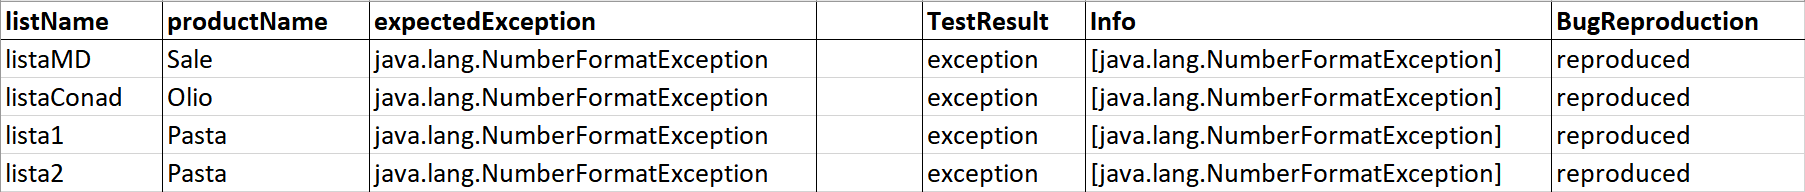
\includegraphics[scale=0.32]{shopping.list.out}
	\centering
			\caption{\emph{output.csv}}
    \label{fig:shopping.list}
\end{figure}
\noindent Come visibile in Figura \ref{fig:shopping.list}, il Framework considera correttamente il bug riprodotto  (BugReproduction='reproduced') quando l'esecuzione del caso di test parametrico fa sollevare l'eccezione specificata in input nella colonna 'expectedException' (TestResult="exception", Info="java.lang.NumberFormatException"). Nell'esempio considerato, l'esecuzione del caso di test solleva sempre l'eccezione attesa indipendentemente dai parametri inseriti dall'utente (il bug non dipende dai valori in input). Quindi l'attività di validazione per questo specifico caso è andata a buon fine.


\subsection{OpenScale}
 \begin{figure}[H]
	
\includegraphics[width=3cm]{open.scale}
	\centering
\end{figure}

\noindent\textbf{Introduzione}\newline
Open Scale è un’applicazione utile a tenere un registro delle metriche del proprio corpo. Supporta funzioni Bluetooth, e può tenere traccia di tutti i dati inseriti in un grafico.\\ (\textcolor{gray}{repository: }https://github.com/oliexdev/openScale)
\\\\
\noindent\textbf{Bug}\newline
Nella relase 1.5, nel momento in cui si vogliono inserire un peso maggiore di 300 o un indice di massa grassa superiore a 40, oppure entrambi, l’applicazione non lo consente (pur essendo valori corretti secondo le specifiche del programma).
\\\\
\noindent\textbf{Caso di test}\newline
Il caso di test prevede l'inserimento di un nuovo  valore per il campo Weight (parametro \emph{weight}) e un nuovo valore per il campo Body fat percentage (parametro \emph{bodyFatPercentage}).
\\\\

\noindent\textbf{Riproduzione del bug}\newline
\noindent\ul{tipologa del bug atteso:} exception (expectedException: 'NoMatchingViewException')\\
\noindent Se l'applicazione solleva l'eccezione 'NoMatchingViewException', allora il bug è stato riprodotto.
\\\\
\noindent\textbf{Validazione}
 \begin{figure}[H]
	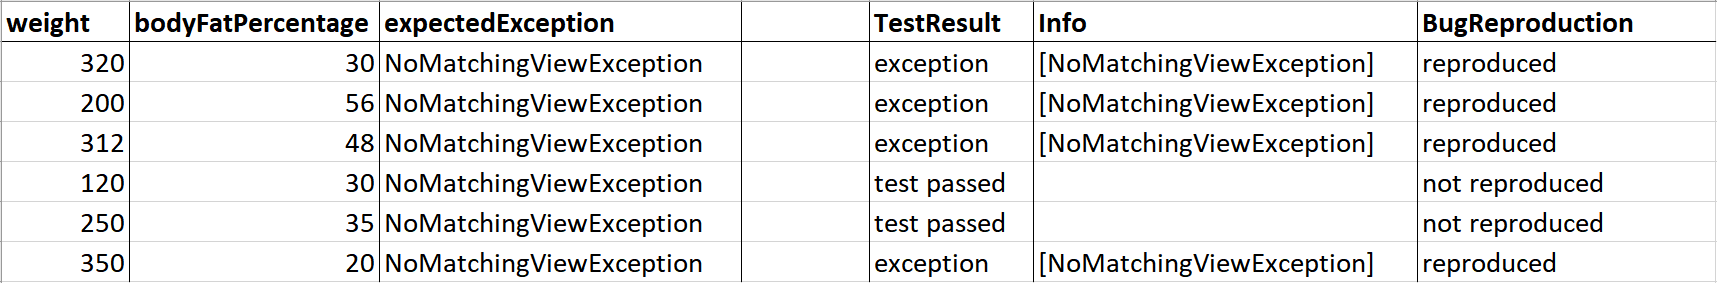
\includegraphics[scale=0.35]{open.scale.out}
	\centering
		\caption{\emph{output.csv}}
    \label{fig:open.scale}
\end{figure}
\noindent Come visibile in Figura \ref{fig:open.scale}, il Framework considera correttamente il bug riprodotto  (BugReproduction='reproduced') quando l'esecuzione del caso di test parametrico fa sollevare l'eccezione specificata in input nella colonna 'expectedException' (TestResult="exception", Info="NoMatchingViewException"). Nell'esempio considerato infatti, quando il caso di test prevede un parametro \emph{weight} maggiore di 300 o un parametro \emph{bodyFatPercentage} maggiore di 40 (o entrambi), viene sollevata l'eccezione attesa e il bug viene riprodotto. Quindi l'attività di validazione per questo specifico caso è andata a buon fine.
